\chapter{Datenbankgestützte Implementierung von CNN}
\label{kap:CNN_in_SQL}
In diesem Kapitel werden Ideen zur Umsetzung der datenbankgestützten Mustererkennung durch trainierte gefaltete neuronale Netze vorgestellt. Der Schlüssel liegt dabei in der effektiven Implementierung der Faltungsoperation als SQL-Anfrage. Gelingt dies, so kann die Vorwärtsrechnung eines CNN durch Komposition von Faltungs-, Pooling- und Matrixvektoroperationen umgesetzt werden. Im Abschnitt \ref{abs:conv_in_sql} werden drei Implementierungsmöglichkeiten der Matrixfaltung, siehe Definition \ref{def:matrix_faltung}, in SQL beleuchtet. Dabei stellt sich heraus, dass es sich lohnt, die diskrete Faltung mit Operationen der linearen Algebra mithilfe der in Kapitel \ref{kap:fund} vorgestellten Basisoperationen umzusetzen. So gelingt es, die Problemstellung \ref{prob:conv_in_sql} zu lösen und auch für relativ große Grauwertbilder akzeptable Laufzeiten zu erreichen, die jedoch in Zukunft noch verbessert werden müssen.

Im Abschnitt \ref{abs_CNN_in_SQL} wird hinsichtlich Problem \ref{prob:ffCCN} eine (objekt-) relationale Umsetzung der Vorwärtsrechnung für das Modell \ref{modell} zur Ziffernerkennung vorgestellt. Dieses Modell sei mithilfe des Backpropagationsalgorithmus \ref{alg:cnn_online} bereits trainiert, siehe Abschnitt \ref{abs:model_mnist}.
\section{Die Faltungsoperation in SQL}
\label{abs:conv_in_sql}
Die Faltung zweier zeitdiskrete Signale stellt die Kernoperation innerhalb von CNN dar. Sind die entsprechenden Signale zweidimensional wie in Problemstellung \ref{prob:conv_in_sql}, so muss die Matrixfaltung $X \ast K$ für $X \in \RR^{h \times b}$ und $K \in \RR^{k \times k}$ mithilfe des im Abschnitt \ref{abs:relation_intro} vorgestellten SQL-Kerns umgesetzt werden. Dazu werden in diesem Abschnitt drei Varianten vorgestellt, welche das Coordinate-Schema bzw. das Spaltenkompression-Schema zur Darstellung der Matrizen $X$ und $K$ nutzen. 
\subsection{Faltung mit Nachbarschaften}
\label{abs:naive_app}
Der erste Ansatz beruht auf den Nachbarschaftsbeziehungen der Pixel innerhalb der Matrix $X$, die durch die Faltung mit einem gedrehten Kern $K$ mit den Abmessungen $k \times k$ gegeben sind. Dazu werden einige Bezeichnungen im Folgenden eingeführt. Seien $l=\lfloor k/2 \rfloor$ und die Mengen
\begin{align*}
    N:=\{(i,j) \; :\; 1 \leq i \leq b, 1 \leq j \leq h \}
\end{align*} 
sowie
\begin{align*}
    F:=\{(i,j) \; :\; -l \leq i \leq l, -l \leq j \leq l \}
\end{align*} 
gegeben, welche die Positionen der Matrizen $X$ und $K$ widerspiegeln. Hier wird wieder die spezielle Indizierung des Kerns $K$ wie in Bemerkung \ref{bem:K_conv_komp} genutzt. Nun kann für jedes Pixel $(i,j)$ von $X$ eine Umgebung $U(i,j)$  in Abhängigkeit von $F$ definiert werden, und zwar
\begin{equation}
    \label{eq:neighborhood}
    U(i,j):=\{(i', j') \; : \; (i'-i, j'-j) \in F \}.
\end{equation}
Die Menge $U(i,j)$ wird auch als Nachbarschaft des Pixels $(i,j)$ bezeichnet.
Die Matrixfaltung $Y= X \ast K$ lässt sich mit den Umgebungen durch
\begin{equation}
    \label{eq:naive_approach}
    Y_{i,j}=\sum_{(i',j') \in U(i,j)} X_{i', j'} K_{i'-i, j'-j}, \; \; \forall i \in [h], \forall j \in [b]
\end{equation}
berechnen. Dabei wird $X$ außerhalb des Definitionsbereiches mit Nullen aufgefüllt, sodass das Ergebnis $Y$ wieder die gleichen Abmessungen wie $X$ besitzt.

Zur Umsetzung der Faltungsoperation sind also zunächst die Nachbarschaften für jedes Pixel von $X$ zu berechnen. In SQL kann dies mithilfe des kartesischen Produkts implementiert werden. Dazu bezeichnen $\mathbf{X}$ und $\mathbf{K}$ die Relation zur Darstellung der Matrizen $X \in \RR^{h \times b}$ und $K \in \RR^{k \times k}$ im Coordinate-Schema. Eine rein relationale Umsetzung von Gleichung (\ref{eq:naive_approach}) ist durch die SQL-Anfrage \ref{sql:naive} gegeben. Zur Übersicht sind die SQL-Operationen blau gekennzeichnet. Als Datenbankmanagementsystem wird PostgreSQL mit der voreingestellten Parameterkonfiguration genutzt. Bestimmte Parameter sind der Tabelle \ref{tab:systemspecs} zu entnehmen. Für eine detailliertere Beschreibung dieser Parameter und deren Bedeutung sei auf die PostgreSQL-Dokumentation verwiesen.

\begin{table}[h]
    \centering
    \begin{tabular}{|l|r|} \hline
        Parameter & Value \\
        \hline
        shared\_buffers &128MB \\
        \hline
        temp\_buffers &8MB \\
        \hline
        effective\_cache\_size &4GB \\
        \hline
        work\_mem &4MB \\
        \hline
        maintenance\_work\_mem &64MB \\
        \hline
        min\_wal\_size &80MB \\
        \hline
        max\_wal\_size &1GB \\
        \hline
        wal\_buffers &4MB \\
        \hline
    \end{tabular}
    \caption[PostgreSQL-Parameterkonfiguration]{Es ist die verwendete Parameterkonfiguration von PostgreSQL 14 dargestellt.}
    \label{tab:systemspecs}
\end{table}

\lstinputlisting[label=sql:naive, caption=SQL-Code zur Umsetzung der Faltung mit Nachbarschaften, language=SQL]{sql_code/neighborhood.sql}

In der Anfrage (Zeile 4-14) werden die Nachbarschaften aller Pixel in der temporären Relation $\mathbf{kreuz}$ berechnet. Dabei wird die \textbf{BETWEEN}-Funktion zur kompakten Darstellung der Konstantenselektion bezüglich $l=\lfloor k/2 \rfloor$ genutzt. In den Zeilen 15-17 werden dann die Nachbarschaften über die entsprechenden Indizes der Matrix $K$ verbunden und schließlich die \textbf{SUM}-Funktion genutzt, um das Faltungsergebnis zu berechnen. Dieser naive Ansatz nutzt keine lineare Algebra in Form von Matrixvektor- oder Matrixmatrixmultiplikation und ist hinsichtlich des Problems \ref{prob:conv_in_sql} schon für verhältnismäßig kleine Grauwertbilder ineffizient. Zu erkennen ist dies in der Abbildung \ref{abb:laufzeit_naive}, bei der die Laufzeiten der SQL-Anfrage \ref{sql:naive} in Abhängigkeit von der Dimension $n$ für allgemeine Matrizen $X \in \RR^{n \times n}$ dargestellt ist.

\begin{figure}[h]
    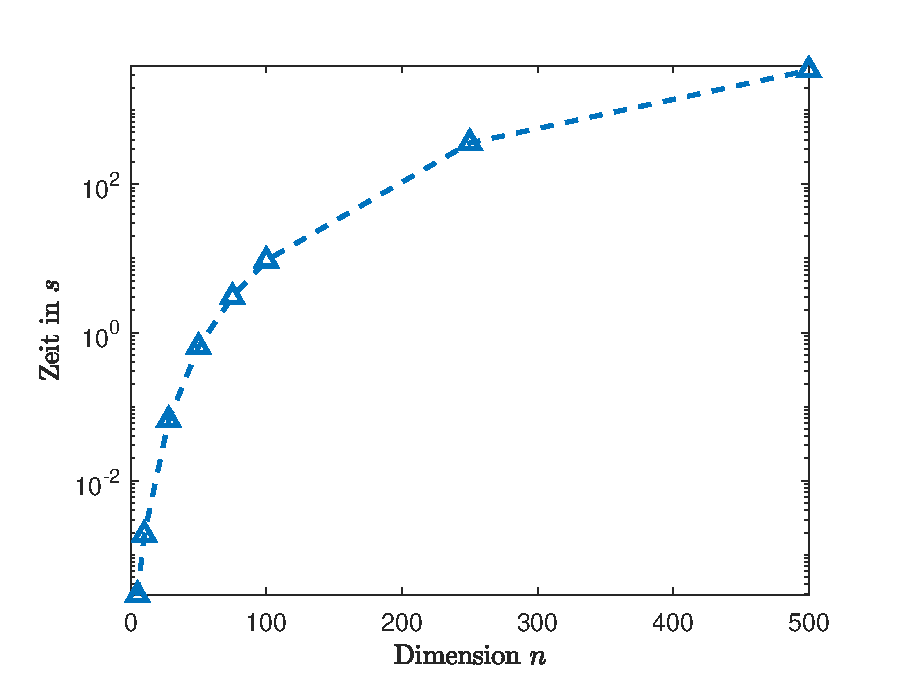
\includegraphics[width=0.8\textwidth]{pics/chapters/kap5/data_plot_naive_verb.eps}
    \centering
    \caption[Laufzeiten des Nachbarschaft-Ansatzes]{Es sind die Laufzeiten der SQL-Anfrage \ref{sql:naive} abhängig von der Größe der Matrix $X \in \RR^{n \times n}$ in Sekunden dargestellt. Dabei wurde PostgreSQL mit der Konfiguration in Tabelle \ref{tab:systemspecs} genutzt.}
    \label{abb:laufzeit_naive}
\end{figure}

Eine Verminderung der Laufzeiten kann mithilfe von Umsetzungstabellen, engl. \textit{Lookup tables}, erreicht werden. Da die Dimensionen aller vorkommenden Merkmalskarten und Kerne eines CNN von Anfang an durch die Wahl der Hyperparameter festgelegt werden, müssen die Nachbarschaften für die Faltung und das Pooling nur einmalig berechnet werden. Dies kann zudem vor der eigentlichen Vorwärtsrechnung durchgeführt werden. So wird zwar der Speicheraufwand erhöht, aber der Zeitaufwand hinsichtlich der Faltungs- und Pooling-Pperation deutlich vermindert. Dazu werden pro Faltungs- und Poolingschicht jeweils eine Umsetzungstabelle \textbf{U} in der Form 
\begin{align*}
    \mathbf{U}( &\underline{i} \; \; \mathrm{int}, \\
    &\underline{j} \; \;\mathrm{int},\\
    &\underline{\text{id}} \; \; \mathrm{int}, \\
    &\text{istrich} \; \; \mathrm{int},\\
    &\text{jstrich}\; \; \mathrm{int})
\end{align*}
mit dem zusammengesetzten Schlüssel $(i,j,\text{id})$ benötigt. Hier werden für jedes Pixel $(i,j)$ die Nachbarpixel $(i', j') \in U$ mit einer entsprechenden Nummer $\text{id}$ zur Identifikation  hinterlegt. So wird die zeitintensive Berechnung der Nachbarschaften mit dem  kartesischen Produkt in der Anfrage \ref{sql:naive} umgangen. Die Laufzeiten der verbesserten Anfrage \ref{sql:naive_better} sind in Abhängigkeit von der Dimension $n$ in Abbildung \ref{abb:laufzeit_naive_verb} dargestellt. Dabei ist der erhöhte Speicheraufwand für die Umsetzungstabellen für einen Kern $K \in \RR^{3 \times 3}$ sichtbar. Kerne mit diesen Abmessungen werden oft in der Praxis verwendet. 

\lstinputlisting[label=sql:naive_better, caption=SQL-Code zur Umsetzung der Faltung mit Umsetzungstabellen, language=SQL]{sql_code/neigh_verbesster.txt}

\begin{figure}[h]
    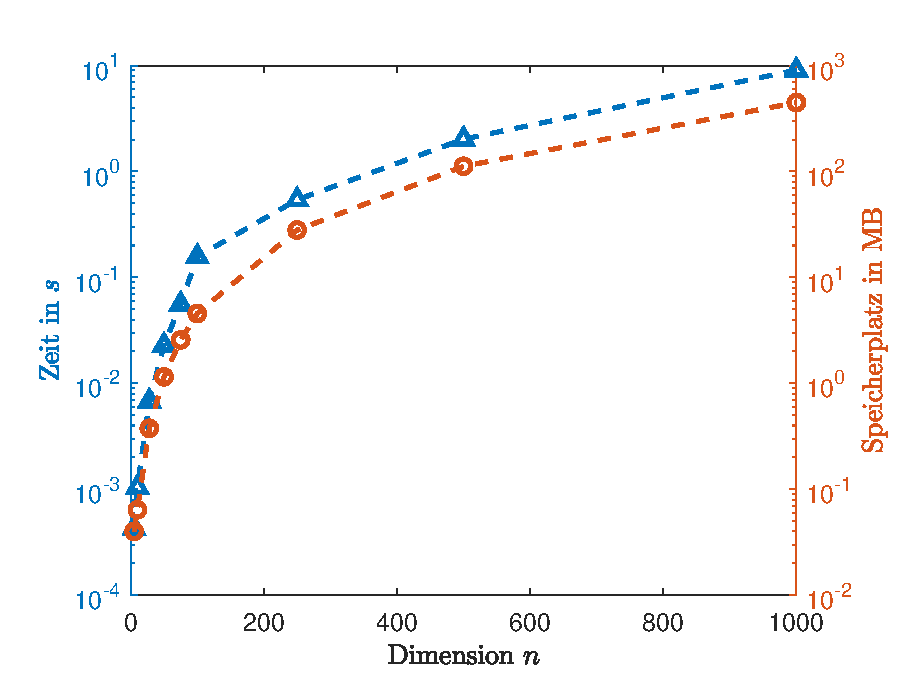
\includegraphics[width=0.8\textwidth]{pics/chapters/kap5/data_plot_naive_verb_verb.eps}
    \centering
    \caption[Laufzeiten und Speicherbedarf bei verbesserter Nachbarschaft]{Es ist der Zeit- und Speicheraufwand der SQL-Anfrage \ref{sql:naive_better} in Abhängigkeit von der Größe der Matrix $X \in \RR^{n \times n}$ dargestellt. Die blaue Kurve spiegelt die Laufzeiten in Sekunden wider. Außerdem ist der benötigte Speicherbedarf der Umsetzungstabellen für die Nachbarschaften in PostgreSQL für einen Kern $K \in \RR^{3 \times 3}$ in MB abgebildet.}
    \label{abb:laufzeit_naive_verb}
\end{figure}

\subsection{Faltung als Matrixvektorprodukt}
\label{abs:conv_using_sparse}
Zwei beliebige Funktionen $f,g: D \rightarrow \mathbb{R}$ mit endlichem Definitionsbereich $D$ können als zeitdiskrete Signale $f=(f_0, \ldots, f_{n-1})^T \in \mathbb{R}^{n}$ und $g=(g_0, \ldots, g_{n-1})^T \in \mathbb{R}^{n}$ aufgefasst werden. %Durch das Fortsetzen mit Nullen besitzen die Vektoren $f$ und $g$ die gleiche Länge. 
Die zyklische Faltung dieser eindimensionalen Signale wird im Folgenden erklärt.

\begin{defi}[Zyklische Faltung]
    \label{def:cycconv}
    Die zyklische Faltung $y=f \circledast g \in \RR^{n}$ zweier zeitdiskreter Signale $f \in \RR^n$ und $g \in \RR^n$ ist durch
    \begin{equation*}
        y_k:=\sum_{j=0}^{n-1} f_j g_{(k-j) \, \mathrm{mod} \; n},  \; \; 0 \leq k \leq n-1
    \end{equation*}
    definiert. Dabei werden Indizes außerhalb von $0, \ldots, n-1$ durch Modulo-Rechnung ($\mathrm{mod} \; n)$ in den gültigen Indexbereich abgebildet.
\end{defi}
In diesem Fall kann die zyklische Faltung von $f$ und $g$ als Matrixvektorprodukt mit speziellen Toeplitz-Matrizen formuliert werden. 

\begin{defi}[Toeplitz-Matrix, Zyklische Matrix]
    \label{def:toeplitzM}
    Eine diagonalkonstante Matrix $A \in \RR^{n \times n}$ der Gestalt
    \begin{equation*}
    A=
    \begin{pmatrix}
        a_0 & a_{-1} &a_{-2} &\ldots &\ldots &a_{-(n-1)} \\ 
        a_1 & a_0 &a_{-1} &\ddots & &\vdots \\
        a_2 & a_1 &\ddots &\ddots &\ddots &\vdots\\
        \vdots & \ddots &\ddots &\ddots &a_{-1} &a_{-2}\\
        \vdots & &\ddots &a_1 &a_0 &a_{-1} \\
        a_{n-1} &\ldots &\ldots &a_{2} &a_{1} &a_0
    \end{pmatrix}
\end{equation*}
    wird Toeplitz\footnote{Otto Toeplitz 1881-1940}-Matrix genannt. Es gilt 
    \begin{equation}
        A_{i,j}=A_{i+1,j+1}=a_{i-j}
    \end{equation}
 für alle Indizes $0 \leq i, j \leq n-1$. Eine quadratische Toeplitzmatrix ist damit durch ihre erste Zeile und Spalte eindeutig bestimmt. Für den Spezialfall $a_i=a_{-(n-i)}=a_{i-n}$ für alle $0 \leq i \leq n-1$ wird $A$ zyklische Matrix genannt. Zyklische Matrizen sind damit eindeutig durch einen Vektor $a \in \RR^n$ charakterisiert.
\end{defi}

%\begin{defi}[Zyklische Matrix, vgl. Gray\cite{gray2006toeplitz}]
  %  \label{def:zykM}
   % Eine quadratische Matrix heißt zyklisch im Vektor $a=(a_0, \ldots, a_{n-1})^T \in \RR^n$, wenn sie die Gesatlt
    %\begin{equation*}
        %\mathrm{zyk}(a):=
        %\begin{pmatrix}
            %a_0 & a_{n-1} &a_{n-2} &\ldots &a_1 \\ 
            %a_1 & a_0 &a_{n-1} & \ldots &a_2 \\
            %a_2 & a_1 &a_0 & \ldots &a_3 \\
            % &\ddots &\ddots &\ddots & \\
            %a_{n-1} &a_{n-2} &a_{n-3} &\ldots &a_0
        %\end{pmatrix}
    %\end{equation*}
   % besitzt.
%\end{defi}    
    
Für zeitdiskrete Signale $f,g \in \mathbb{R}^{n}$ kann die zyklische Faltung $y=f \circledast g$ als Matrixvektorprodukt mit einer zyklischen Matrix dargestellt werden. Es gilt 
\begin{equation*}
    y=\underbrace{\begin{pmatrix}
        g_0 & g_{n-1} &g_{n-2} &\ldots &g_1 \\ 
        g_1 & g_0 &g_{n-1} &\ldots &g_2 \\
        g_2 &g_1 &g_0 &\ddots &g_3\\
        &\ddots &\ddots &\ddots & & \\
        g_{n-1} &g_{n-2} &g_{n-3} &\ldots &g_0
    \end{pmatrix}}_{=:\mathrm{zyk}(g)}
    \begin{pmatrix}
        f_0 \\
        f_1 \\
        f_2 \\
        \vdots \\
        \vdots \\
        f_{n-1}
    \end{pmatrix}
\end{equation*}
Die Faltung zweidimensionaler Signale kann mithilfe von doppelt zyklischen Blockmatrizen dargestellt werden.
    %Matrix im Vektor $f$. Sei weiter $g \in \mathbb{R}^{n}$. Dann lässt sich mit
%\begin{equation*}
 %       (F g)_k=\sum_{j=0}^{n-1}  f_{k-j} g_j,  \; \; k=0, \ldots, n-1
  %  \end{equation*}
   % die diskrete Faltung von $f$ und $g$ darstellen. Dabei werden Indizies außerhalb von $0, \ldots, n-1$ zyklisch durch Modulo-Rechnung ($\mathrm{mod} \; n)$ in den gültigen Indexbereich abgebildet. Zyklische Matrizen aus Definition \ref{def:zykM} stellen Spezialfälle von Toeplitz-Matrizen dar.
\begin{defi}[Doppelt zyklische Blockmatrix]
    \label{def:double_circ}
    Eine Blockmatrix $A \in \RR^{n^2 \times n^2}$ bestehend aus Blockmatrizen $B_{i,j} \in \RR^{n \times n}$ heißt zyklische Blockmatrix genau dann wenn, die Matrizen $B_{i,j}$ für alle $ 1 \leq i, j \leq n$ zyklisch im Sinne von Definition \ref{def:toeplitzM} sind. Ist zusätzlich $A$ eine zyklische Matrix, so wird $A$ doppelt zyklische Blockmatrix genannt.
\end{defi}

Die Konstruktion solcher zyklischen Blockmatrizen soll im Folgenden beleuchtet werden. Dazu seien die Matrizen $X \in \RR^{n \times n}$ und $K \in \RR^{k \times k}$ gegeben. Zunächst wird der Kern $K$ in eine $n \times n$-Matrix eingebettet, die wieder mit $K \in \RR^{n \times n}$ bezeichnet wird. Dazu wird der Kern von unten und von rechts mit Nullen aufgefüllt, siehe Beispiel \ref{bsp:Kzeropad}.
Weiter bezeichne $\mathrm{vec}(X)$ die Transformation der Matrix $X$ in einen Vektor der Länge $n^2$, indem die Spalten von $X$ untereinander geschrieben werden, ähnlich wie bei der Flatten-Funktion, vgl. Definition \ref{def:flatten}. Das folgende Lemma liefert die Darstellung der Matrixfaltung, siehe Bemerkung \ref{bem:K_conv_komp}, als Matrixvektorprodukt mit dünnbesetzter Matrix.

\begin{lem}[vgl. Jain \cite{jain1989fundamentals}, \cite{DBLP:journals/corr/abs-1805-10408}]
    Für einen gedrehten Kern $K \in \RR^{n \times n}$ wird die zyklische Blockmatrix $A \in \RR^{n^2 \times n^2}$ als
    \begin{equation*}
        A=\begin{bmatrix}
            \mathrm{zyk}(K_{1,:}) &\mathrm{zyk}(K_{2,:}) &\ldots &\mathrm{zyk}(K_{n,:}) \\
            \mathrm{zyk}(K_{n,:}) &\mathrm{zyk}(K_{1,:}) &\ldots & \; \; \;\mathrm{zyk}(K_{n-1,:})\\
            \vdots &\vdots &\ddots &\vdots\\
            \mathrm{zyk}(K_{2,:}) &\mathrm{zyk}(K_{3,:}) &\ldots &\mathrm{zyk}(K_{1,:})
        \end{bmatrix}
    \end{equation*}
    konstruiert. Sei die zweidimensionale Faltung von $X$ und $K$ als
    \begin{equation*}
        Y_{i,j}= \sum_{u=0}^{n-1} \sum _{v=0}^{n-1} X_{i+u,j+v} K_{u,v} 
    \end{equation*}
    mit $X_{i,j}=0$ für $i \notin\{0,\ldots, n-1\}$ und $j \notin \{0, \ldots, n-1\}$ gegeben. Dann gilt der Zusammenhang
    $\mathrm{vec}(Y)=A \, \mathrm{vec}(X)$. Die Matrix $A$ ist dünnbesetzt. 
\end{lem}

\begin{proof}
    Ein Beweis ist von Jain \cite{jain1989fundamentals} gegeben. Das Auffüllen von $K \in \RR^{k \times k}$ zu $K \in \RR^{n \times n}$ mit Nullen führt zur dünnbesetzten Struktur der Matrix $A$. 
\end{proof}
\begin{bsp}
    \label{bsp:Kzeropad}
    Seien die Matrizen
    \begin{equation*}
        X=\begin{pmatrix}
            x_1 & x_2 &x_3 \\
            x_4 & x_5 &x_6 \\
            x_7 & x_8 &x_9 \\
        \end{pmatrix}, \; \;
        K=\begin{pmatrix}
            k_1 & k_2 &0\\
            k_3 &k_4 &0 \\
            0 &0 &0
        \end{pmatrix}
    \end{equation*}
    gegeben. Mit 
    \begin{align*}
    A \, \mathrm{vec}(X) &=    
    \begin{pmatrix}
        k_1 & k_2 & 0 &k_3 &k_4 &0 &0 &0 &0 \\
        0 & k_1 & k_2 &0 &k_3 &k_4 &0 &0 &0 \\
        0 & 0 & 0 &k_1 &k_2 &0 &k_3 &k_4 &0 \\
        0 & 0 & 0 &0 &k_1 &k_2 &0 &k_3 &k_4 
    \end{pmatrix}
    \begin{pmatrix}
        x_1 \\
        x_2 \\
        x_3 \\
        x_4 \\
        x_5 \\
        x_6 \\
        x_7 \\
        x_8 \\
        x_9
    \end{pmatrix} \\
    &=\begin{pmatrix}
        k_1 x_1+ k_2 x_2 +k_3 x_4 +k_4 x_5 \\
        k_1 x_2+ k_2 x_3 +k_3 x_5 +k_4 x_6 \\
        k_1 x_4+ k_2 x_5 +k_3 x_7 +k_4 x_8 \\
        k_1 x_5+ k_2 x_6 +k_3 x_8 +k_4 x_9 
    \end{pmatrix}=\mathrm{vec} \, (Y)
\end{align*}
kann die Matrixfaltung $Y = X \ast K$ ohne zero padding, welche im Modell \ref{modell} benötigt wird, berechnet werden. Dazu muss lediglich der Vektor $\mathrm{vec}(X)$ in eine entsprechende Matrix transformiert werden.
\end{bsp}
Im Beispiel \ref{bsp:Kzeropad} ist zu beachten, dass $A$ keine doppelt zyklische Blockmatrix ist, da sich die Abmessungen der Ergebnismatrix $ Y \in \RR^{2 \times 2}$ mit der gültigen Faltung verkleinern. Es fehlen also gewisse Zeilen in $A$, sodass $A$ nicht zyklisch ist.
Die genaue Konstruktion doppelt zyklischer Blockmatrizen für die Faltungsoperation mit bzw. ohne zero padding ist ein technisches Detail und wird in dieser Arbeit nicht weiter beleuchtet. Für eine mögliche Implementierung sei auf den MATLAB-Code \ref{mat:code:zyk} im Anhang \ref{app:app_2}verwiesen. 

Die datenbankgestützte Umsetzung der Matrixvektormultiplikation mit dünnbesetzter Matrix wurde bereits im Abschnitt \ref{abs:SQL_linalg} erläutert. Bei CNN lassen sich die dünnbesetzten zyklischen Blockmatrizen für die Kerne bereits vor der Vorwärtsrechnung in Relationen speichern. Seien $X \in \RR^{n \times n}$ und $K \in \RR^{k \times k}$ sowie \textbf{vecX} und \textbf{K} entsprechende Relationen des Vektors $\mathrm{vec}(X)$ bzw. der eingebetteten $n \times n$-Matrix $K$ im Coordinate-Schema. Die Matrixfaltung $Y = X \ast K$ lässt sich mit den obigen Resultaten in der SQL-Anfrage \ref{sql:sparseapp} berechnen. In der Abbildung \ref{abb:sparseapp} sind numerische Resultate hinsichtlich des Speicher- und Zeitaufwands der SQL-Anfrage \ref{sql:sparseapp} für einen Kern $K \in \RR^{3 \times 3}$ dargestellt.

\begin{figure}[h]
    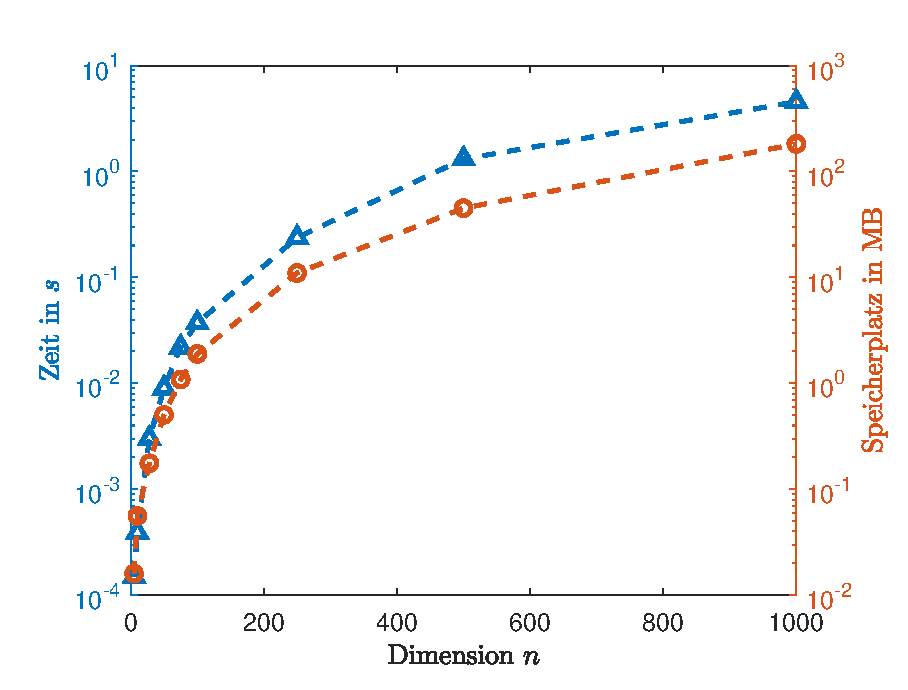
\includegraphics[width=0.8\textwidth]{pics/chapters/kap5/data_plot_sparse_ver.eps}
    \centering
    \caption[Laufzeiten und Speicherbedarf der \textit{sparse}-Variante]{Es ist der Zeit- und Speicheraufwand der SQL-Anfrage \ref{sql:sparseapp} in Abhängigkeit von der Größe der Matrix $X \in \RR^{n \times n}$ dargestellt. Die blaue Kurve spiegelt die Laufzeiten in Sekunden wider. Außerdem ist der benötigte Speicherbedarf der dünnbesetzten Matrizen im Spaltenkompression-Schema für einen Kern $K \in \RR^{3 \times 3}$ in MB abgebildet.}
    \label{abb:sparseapp}
\end{figure}

\lstinputlisting[label=sql:sparseapp, caption=SQL-Code zur Umsetzung der Matrixfaltung als Matrixvektorprodukt, language=SQL]{sql_code/sparsecnn.txt}

\subsection{Diskrete Fourier-Transformation}
\label{abs:dft}
Die diskrete Fourier\footnote{Jean Baptiste Joseph Fourier 1786-1830}-Transformation ist eine Methode aus dem Bereich der Fourier-Analysis. Dabei werden zeitdiskrete, endliche Signale auf sogenannte diskrete, periodische Frequenzspektren abgebildet. In diesem Kontext wird zwischen Zeitbereich und Frequenzbereich unterschieden.

\begin{defi}[Diskrete Fourier-Transformation]
    \label{def:dft}
    Im Zeitbereich sei ein diskretes Signal $x=(x_0, \ldots, x_{n-1})^T \in \RR^n$ gegeben. Dann wird mit $\hat{x}=(\hat{x}_0, \ldots, \hat{x}_{n-1}) \in \mathbb{C}^n$ das Ergebnis der diskreten Fourier-Transformation, kurz $\hat{x}=\mathrm{DFT}(x)$, bezeichnet. Die sogenannten Fourier-Koeffizienten sind als 
    \begin{equation*}
        \hat{x}_k:=\sum_{j=0}^{n-1} \mathrm{e}^{- \frac{2 \pi i}{n} j k} \cdot x_j
    \end{equation*}
    für $0 \leq k \leq n-1$ definiert. Das komplexe Signal $\hat{x}$ ist dem Frequenzbereich zugeordnet.
\end{defi}
Mit der inversen Fourier-Transformation kann aus dem Signal im Frequenzbereich das Signal im Zeitbereich rekonstruiert werden. Damit ist es möglich, Signale im Frequenzbereich zu manipulieren und zwischen Zeit- und Frequenzbereich beliebig zu wechseln.
\begin{defi}[Inverse diskrete Fourier-Transformation]
    Sei $\hat{x}=(\hat{x}_0, \ldots, \hat{x}_{n-1}) \in \mathbb{C}^n$. Mit den Koeffizienten
    \begin{equation*}
        x_j:= \frac{1}{n} \sum_{k=0}^{n-1} \mathrm{e}^{\frac{2 \pi i}{n} j k} \cdot \hat{x}_k, \; \; 0 \leq j \leq n-1
    \end{equation*}
    lässt sich die inverse diskrete Fourier-Transformation, kurz $x=\mathrm{iDFT}(\hat{x})$, angeben. Das Paar $(x ,\hat{x})$ wird Fourier-Paar genannt.
\end{defi}
Die diskrete Fourier-Transformation aus Definition \ref{def:dft} lässt sich in ein Matrixvektorprodukt $\hat{x}=Fx$ überführen, wobei $F \in \mathbb{C}^{n \times n}$ eine symmetrische Matrix der Gestalt
\begin{equation}
    \label{eq:FM}
    F=\begin{pmatrix}
        &1 &1 &1 &\ldots &1 \\
        &1 &\omega_n &\omega_n^2 &\ldots &\omega_n^{(n-1)} \\
        &1 &\omega_n^2 &\omega_n^4 &\ldots &\omega_n^{2 (n-1)} \\
        &\vdots &\vdots & &\ddots &\vdots \\
        &1 &\omega_n^{(n-1)} &\omega_n^{2(n-1)}  &\ldots &\omega_n^{(n-1)(n-1)}
    \end{pmatrix}
\end{equation}
mit 
\begin{equation*}
    \omega_n^{j}:=\mathrm{e}^{- \frac{2 \pi i}{n} j}, \; \; 0 \leq j \leq n-1
\end{equation*}
ist. Diese Matrix wird Fourier-Matrix genannt und deren Einträge $\omega_n^{j}$ als $n$-te Einheitswurzeln bezeichnet. Es gilt $\omega_n^n=1$.
\begin{lem}
    \label{lem:Finv}
    Es gilt $F^*=\bar{F}$ und die Matrix $\frac{1}{\sqrt{n}} F$ ist unitär. Für $x \in \RR^n$ sei $\hat{x}=Fx$. Dann gilt $F^{-1}=\frac{1}{n} \bar{F}$ und $x= \frac{1}{n}\bar{F} \hat{x}$.
\end{lem}
\begin{proof}
    Wegen $F=F^T$ gilt 
    \begin{equation*}
        F^*=\bar{{F}}^T=\bar{F}.
    \end{equation*}
    Mit $W:=F\bar{F}$ gilt $W_{k,j}=\sum_{l=0}^{n-1} \omega_n^{(j-k)l}$. Ist $k=j$ so ergeben sich die Einträge auf der Hauptdiagonalen von $W$ zu $n$. Ist $k \neq j$, so ist $\omega_0:=\omega_n^{j-k} \neq 1$ eine $n$-te Einheitswurzel.
    Mit der geometrischen Summenformel gilt
    \begin{equation*}
        W_{k,j}=\sum_{l=0}^{n-1} \omega_0^l=\frac{1-\omega_0^n}{1-\omega_0}=0.
    \end{equation*} 
    Also ist $\left(\frac{1}{\sqrt{n}}\right) F\left(\frac{1}{\sqrt{n}}\right) F^*=I$ und damit $\frac{1}{\sqrt{n}} F$ unitär. Schließlich gilt $\frac{1}{n} \bar{F} F=\frac{1}{n} F \bar{F}= I$ und damit $\hat{x}=Fx \Leftrightarrow \frac{1}{n}\bar{F} \hat{x}=x$.
\end{proof} 
Die inverse diskrete Fourier-Transformation lässt sich mithilfe der diskreten Fourier-Transformation berechnen. Dieser Zusammenhang wird insbesondere für die spätere datenbankgestützte Implementierung der Fourier-Transformationen genutzt.
\begin{lem}
    \label{lem:inversedftasdft}
    Sei das Fourier-Paar
    \begin{align*}
        \mathrm{DFT}(x)&: \; \;\hat{x}_k=\sum_{j=0}^{n-1} \mathrm{e}^{- \frac{2 \pi i}{n} j k} \cdot x_j, \\ 
        \mathrm{iDFT}(\hat{x})&:\; \; x_j= \frac{1}{n} \sum_{k=0}^{n-1} \mathrm{e}^{\frac{2 \pi i}{n} j k} \cdot \hat{x}_k
    \end{align*}
    für $x=(x_0, \ldots, x_{n-1})^T \in \mathbb{R}^n$ gegeben. Dann gilt $x=\frac{1}{n} (DFT(\hat{x}^*))^*$. Hierbei ist mit ${}^*$ die komplexe Konjugation gemeint.
\end{lem}
\begin{proof}
  Für alle $0 \leq j \leq n-1$  gilt
  \begin{align*}
    x_j^{*}&=\frac{1}{n} \sum_{k=0}^{n-1} \mathrm{e}^{-\frac{2 \pi i}{n} j k} \cdot \hat{x}^*_k \\
    &=\frac{1}{n} \mathrm{DFT}(\hat{x}^*)_j.
  \end{align*}
  Die Konjugation auf beiden Seiten liefert die Aussage.
\end{proof}
Wird ein zweidimensionales diskretes Signal in Form einer Matrix $X \in \RR^{n \times n}$ betrachtet, lässt sich die zweidimensionale diskrete Fourier-Transformation definieren. 
\begin{defi}
    Die zweidimensionale diskrete Fourier-Transformation für $X \in \RR^{n \times n}$, kurz $\hat{X}=2\mathrm{DFT}(X)$, ist als
    \begin{align*}
        \hat{X}_{u,v}:&= \sum_{l=0}^{n-1} \sum_{j=0}^{n-1} X_{l,j} \cdot \mathrm{e}^{\frac{2 \pi i}{n} -(lu+jv)} \\
        &=\sum_{l=0}^{n-1} \mathrm{e}^{-\frac{2 \pi i}{n} l u} \left(\sum_{j=0}^{n-1} X_{l,j} \cdot \mathrm{e}^{-\frac{2 \pi i}{n} j v}\right), \; \; 0 \leq u, v \leq n-1
    \end{align*}
    definiert.
\end{defi}
Die zweidimensionale diskrete Fourier-Transformation ist als Hintereinanderausführung von zwei eindimensionalen Fourier-Transformationen, vgl. Definition \ref{def:dft}, zu verstehen. Zuerst wird die $\mathrm{DFT}$ der Zeilen und anschließend die $\mathrm{DFT}$ der Spalten von $X$ berechnet. So lässt sich $\hat{X}=FXF^T$ als Matrixmatrixprodukt mit der Matrix $F$ aus Gleichung (\ref{eq:FM}) darstellen.

Zwischen der zyklischen Faltung aus Definition \ref{def:cycconv} und der diskreten Fourier-Transformation wie in Definition \ref{def:dft} besteht ein fundamentaler Zusammenhang, und zwar das Faltungstheorem. Eine Version davon wird im weiteren Verlauf dieser Arbeit genutzt, um die Matrixfaltung, vgl. Definition \ref{def:matrix_faltung}, mithilfe von Fourier-Transformationen zu berechnen.

\begin{satz}[Zyklisches Faltungstheorem]
    \label{satz:conv_theorem}
    Seien Vektoren $f,g \in \RR^{n}$ gegeben und $y= f \circledast g$ das Ergebnis der zyklischen Faltung. Dann gilt
    \begin{equation}
        \mathrm{DFT}(y)=\mathrm{DFT}(f) \odot \mathrm{DFT}(g).
    \end{equation}
    Dabei bezeichne $\odot$ die elementweise Multiplikation der Einträge von den beteiligten Vektoren.
\end{satz}
\begin{proof}
    Ein Beweis ist von Smith \cite{smith2007mathematics} gegeben.
\end{proof}
\begin{bem}
    Seien die Matrizen $X \in \RR^{n \times n}$ und $K \in \RR^{k \times k}$ mit ungeradem $k$ gegeben. Weiter sei der Kern $K$ gedreht und $l=\lfloor k/2 \rfloor$. Die Matrixfaltung $Y= X \ast K$ ist durch
    \begin{equation*}
        Y_{i,j}=\sum_{u=-l}^l \sum_{v=-l}^l X_{i+u, j+v} K_{u,v}, \; \; 1 \leq i, j \leq n
    \end{equation*}
    erklärt, vgl. Bemerkung \ref{bem:K_conv_komp}.
    Der Kern $K$ wird in eine $n \times n$-Matrix ähnlich wie in Beispiel \ref{bsp:Kzeropad} eingebettet und diese wird wieder mit $K \in \RR^{n \times n}$ bezeichnet wird. In der Matrix $K$ werden zusätzlich bestimmte Zeilen zyklisch verschoben, sodass die zyklischen Randbedingungen der Faltung im Zeitbereich eingehalten werden. Stehen die zweidimensionalen diskreten Fourier-Transformationen $\hat{X}=\mathrm{2DFT}(X)$ und $\hat{K}=\mathrm{2DFT}(K)$ zur Verfügung, so gilt mit dem Faltungstheorem, siehe Satz \ref{satz:conv_theorem}, der Zusammenhang
    \begin{align*}
        \mathrm{2DFT}(Y)&=\mathrm{2DFT}(X) \odot \mathrm{2DFT}(K). 
        %\Leftrightarrow &=\mathrm{i2DFT}(\hat{X} \odot \hat{K}).
    \end{align*}
    % bereits um 180 Grad gedreht, vgl. Bemerkung \ref{bem:K_conv_komp}, 
\end{bem}
Für eine detailliertere Beschreibung der Konstruktion der eingebetteten Matrizen $K \in \RR^{n \times n}$ sei aufgrund deren Umfangs auf Jain \cite{jain1989fundamentals} verwiesen. Eine Implementierungsmöglichkeit \ref{matlab:boundary} in MATLAB ist im Anhang \ref{app:app_2} gegeben.
Die Matrixfaltung innerhalb einer Faltungsschicht eines CNN lässt sich mit den obigen Resultaten in drei Schritten berechnen.
\begin{itemize}
    \item[1.] Es sind jeweils die zweidimensionalen diskreten Fourier-Transformationen $\hat{X}$ und $\hat{K}$ für die Eingabe $X$ und den gedrehten Kern $K$ zu berechnen.
    \item[2.] Die Matrix $\hat{Y}= \hat{X} \odot \hat{K}$, welche sich aus der elementweisen Multiplikation ergibt, ist zu bestimmen.
    \item[3.] Schließlich stellt $Y=\mathrm{i2DFT}(\hat{Y})$ die Matrixfaltung dar, welche mithilfe der inversen diskreten Fourier-Transformation ermittelt wird.    
\end{itemize} 
Für Schritt 1 und Schritt 3 kann wegen Lemma \ref{lem:Finv} und Lemma \ref{lem:inversedftasdft} die Fourier-Matrix $F$ benutzt werden. Die Aufgabe besteht nun darin, die Berechnungen in Algorithmus \ref{alg:conv_as_2dft} datenbankgestützt umzusetzen. 
\begin{algorithm}[h]
    \caption{Matrixfaltung mit diskreten Fourier-Transformationen}
    \label{alg:conv_as_2dft}
    \begin{algorithmic}
    \Require  Eingabematrix $X \in \RR^{n \times n}$, eingebetteter Kern $K \in \RR^{n \times n}$, Fourier-Matrix $F \in \RR^{n \times n}$ 
    \Ensure Matrixfaltung $Y= X \ast K$
    \State Berechne $\mathrm{2DFT}(X)$
    \State $\hat{X}=F X F^T$
    \State $\hat{K}=F K F^T$ 
    \State Berechne das Produkt mit der elementweisen Multiplikation
    \State $\hat{Y}= \hat{X} \odot \hat{K}$
    \State Bestimme $\mathrm{i2DFT}(Y)$
    \State $Z=\hat{Y}^*$
    \State $\hat{Z}=F Z F^T$
    \State $Y=\frac{1}{n^2}\hat{Z}^*$
    \end{algorithmic}
\end{algorithm}

Dies gelingt, da ausschließlich Basisoperationen wie die Matrixmatrixmultiplikation sowie das Adjungieren von Matrizen benötigt werden. Die elementweise Multiplikation und die Konjugation können als einfache skalare Funktionen implementiert werden. Da die Matrix $F$ nur von den Dimensionen der beteiligten Matrizen abhängt und diese durch die Hyperparameter des verwendeten CNN festgelegt sind, kann $F$ vor der Vorwärtsrechnung in einer Relation gespeichert werden. 
Die Matrix $F$ besitzt komplexwertige Einträge und daher wird das Attribut \textbf{v} im Coordinate-Schema in die Attribute \textbf{re} und \textbf{im} aufgeteilt, um den Real- und Imaginärteil getrennt zu speichern. Die Multiplikation zweier komplexer Zahlen $z_1$ und $z_2$ ist durch
\begin{align*}
    z_1 \cdot z_2 &=(\Re(z_1)+ i \Im(z_1))(\Re(z_2)+i \Im(z_2))\\
    &=(\Re(z_1) \cdot \Re(z_2)-\Im(z_1) \cdot \Im(z_2))+ i (\Re(z_1) \cdot \Im(z_2)+ \Im(z_1) \cdot \Re(z_2))
\end{align*}
erklärt.
Darüber hinaus können auch die Fourier-Transformierten $\hat{K}$ für alle beteiligten Kerne $K$ bereits vor der Erkennungsphase bestimmt werden. So kann die Berechnungszeit verkürzt werden.

Seien $X \in \RR^{n \times n}$ und \textbf{X} sowie \textbf{F} Relationen zur Darstellung der Matrizen $X$ und $F$ im Coordinate-Schema. Im ersten Berechnungsschritt ist lediglich die Matrix $\mathrm{2DFT}(X)$ zu bestimmen. Die entsprechende SQL-Anfrage \ref{sql:dft} lässt sich formulieren. Dabei werden \textit{Common-Table-Expressions}, zu Erkennen am Schlagwort \textbf{WITH}, welche als temporäre Tabellen zu verstehen sind, verwendet. So ist es möglich, zum einen Zwischenergebnisse übersichtlich darzustellen und zum anderen jene Ergebnisse weiterzuverwenden. Damit gelingt die iterative Berechnung der Matrixmatrixprodukte. Die erste temporäre Tabelle \textbf{FT}
in den Zeilen 1-6 ermittelt die Matrix $F^T$. In den Zeilen 7-15 wird die Matrix $X F^T$ und anschließend in den Zeilen 16-24 das Produkt $F X F^T$ in der temporären Relation \textbf{FXFT} berechnet. 
Schließlich folgt in den letzten Zeilen die Ausgabe der zweidimensionalen diskreten Fourier-Transformation. Numerische Resultate zum Zeit- und Speicheraufwand der Anfrage \ref{sql:dft} für einen Kern $K \in \RR^{3 \times 3}$ sind der Abbildung \ref{abb:dft_insql} zu entnehmen.

\begin{figure}[h]
    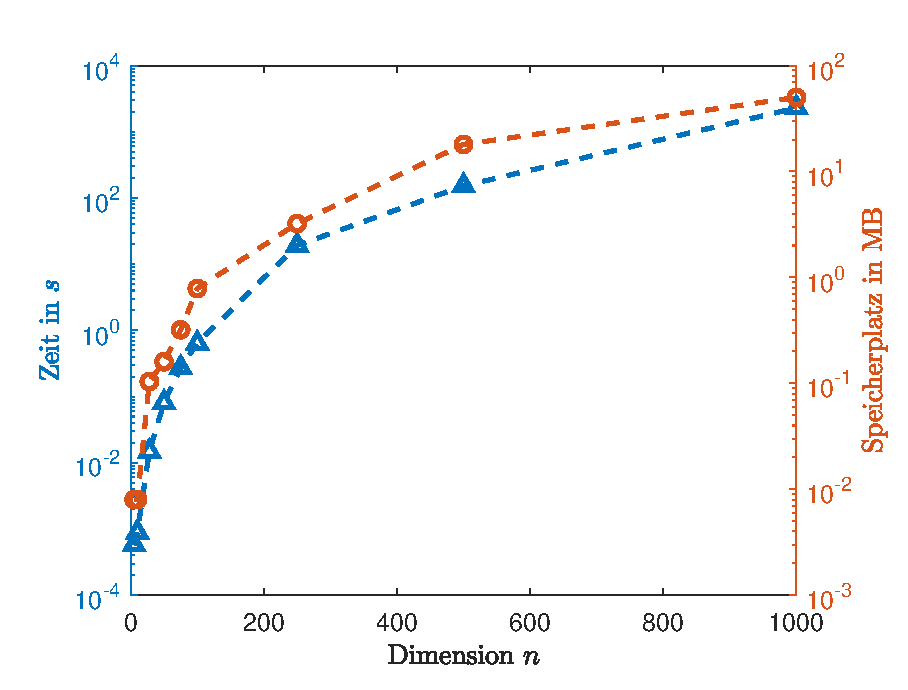
\includegraphics[width=0.8\textwidth]{pics/chapters/kap5/data_plot_2dft_ver.eps}
    \centering
    \caption[Zeit- und Speicheraufwand des $\mathrm{2DFT}$-Ansatzes]{Es ist der Zeit- und Speicheraufwand der SQL-Anfrage \ref{sql:dft} in Abhängigkeit von der Größe der Matrix $X \in \RR^{n \times n}$ dargestellt. Die blaue Kurve spiegelt die Laufzeiten in Sekunden wider. Außerdem ist der benötigte Speicherbedarf der Fourier-Matrizen in PostgreSQL in MB abgebildet.}
    \label{abb:dft_insql}
\end{figure}

%\noindent \begin{minipage}{\linewidth}
    \lstinputlisting[label=sql:dft, caption=SQL-Code zur Umsetzung der $\mathrm{2DFT}$, language=SQL]{sql_code/dft_ansatz_FXFT.txt}
%\end{minipage}

Im zweiten Berechnungsschritt ist eine elementweise Multiplikation auszuführen. Angenommen die Matrizen $\hat{X}$ und $\hat{K}$ sind als Relationen \textbf{X}
und \textbf{K} im Coordinate-Schema hinterlegt. Dann wird $\hat{X} \odot \hat{K}$ in der SQL-Anfrage \ref{sql:elementweise} implementiert. Diese Berechnung ist im Vergleich zur Faltungsoperation nicht zeitkritisch.
Der dritte Berechnungsschritt lässt sich analog zum ersten Schritt darstellen. Dabei ist an zwei Stellen lediglich das Adjungieren einer komplexen Matrix, siehe Anhang \ref{app:app_1}, notwendig.

\lstinputlisting[label=sql:elementweise, caption=SQL-Code zur Umsetzung der elementweisen Multiplikation, language=SQL]{sql_code/dft_ansatz_elemwise.txt}

Wird zur Berechnung der DFT die sogenannte schnelle Fourier-Transformation (engl. \textit{Fast-Fourier-Transformation}, kurz: FFT) genutzt, können die Zeitkosten von $\mathcal{O}(n^2)$ auf $\mathcal{O}(n \log n)$ vermindert werden. In dieser Arbeit wird ausschließlich die diskrete zweidimensionale Fourier-Transformation behandelt. 

\subsection{Zusammenfassung}
\label{abs:sum_conc_in_sql}
In den vorherigen Abschnitten werden drei Ansätze zur datenbankgestützten Umsetzung der Matrixfaltung in SQL beschrieben. Es ist festzuhalten, dass der Nachbarschaft-Ansatz nur mit zugehörigen Umsetzungstabellen für die Umgebungen sinnvoll einsetzbar ist. So wird eine Verminderung der Laufzeit erreicht, aber die benötigten Umsetzungstabellen werden für wachsende Dimensionen schnell größer. Für einen Kern $K \in \RR^{3 \times 3}$ und eine Matrix $X \in \RR^{n \times n}$ ergeben sich  
\begin{equation*}
    \underbrace{16}_{\text{Eckpunkte}}+\underbrace{(4\cdot(n-2))}_{\text{Randpunkte}} \cdot 6 +\underbrace{((n-2)(n-2))}_{\text{innere Punkte}} \cdot 9
\end{equation*}
Tupel in der Umsetzungstabelle.

Der zweite Ansatz nutzt die Darstellung der Faltungsoperation als Matrixvektorprodukt mit dünnbesetzter Matrix. Hinsichtlich der Laufzeiten ist dieser Ansatz am besten geeignet. Jedoch ist auch hier der Speicherbedarf für die Matrizen groß, da die Dimension $n$ bei der Konstruktion der zyklischen Blockmatrizen quadratisch eingeht. 

Im vorherigen Abschnitt \ref{abs:dft} wird die Nutzung der zweidimensionalen diskreten Fourier-Transformation diskutiert. Die datenbankgestützte Umsetzung der zweidimensionalen Fourier-Transformation gelingt mithilfe der Matrixmatrixmultiplikation. Dabei werden Fourier-Matrizen genutzt, die vor der Vorwärtsrechnung in Relationen gespeichert werden können. Mit dem zyklischen Faltungstheorem, vgl. Satz \ref{satz:conv_theorem}, ist die Matrixfaltung mit der $\mathrm{2DFT}$ darstellbar. Hinsichtlich der Laufzeiten schneidet das Verfahren jedoch am schlechtesten ab. Hier könnte die Implementierung der schnellen Fourier-Transformation eine deutliche Verbesserung bewirken. Der Vergleich der Zeit- und Speicherkosten der drei Verfahren zur Berechnung der Matrixfaltung ist in den Abbildungen \ref{abb:vergleich_t} bzw. \ref{abb:vergleich_disk} dargestellt. Je nach Anwendungsszenario und Rahmenbedingungen ist eine entsprechende Vorgehensweise zu wählen.

\begin{figure}[h]
    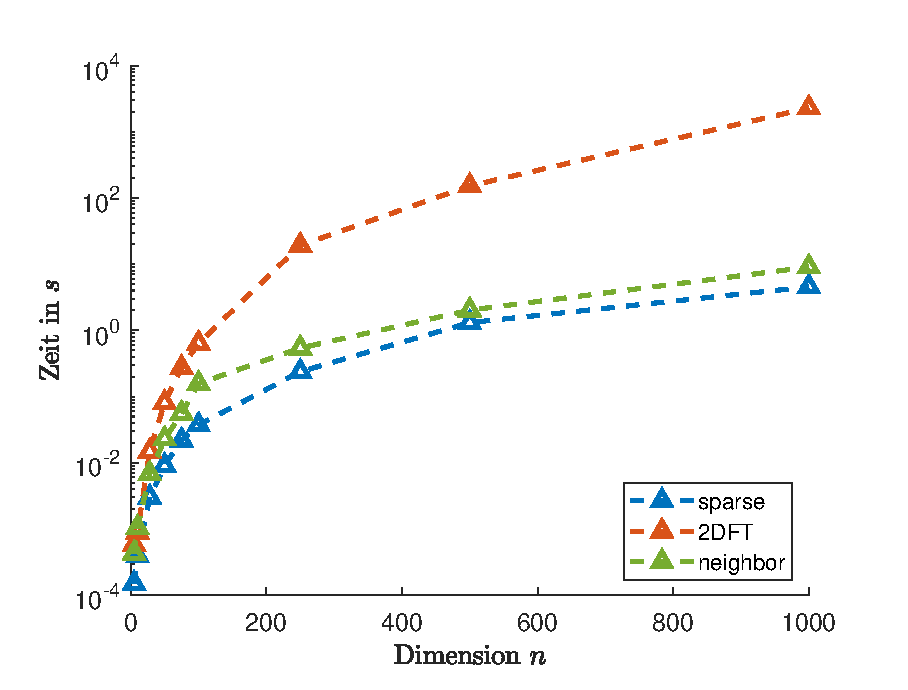
\includegraphics[width=0.8\textwidth]{pics/chapters/kap5/data_plot_vergleich_t.eps}
    \centering
    \caption[Vergleich der Zeitkosten für die Matrixfaltung]{Es sind die Zeitkosten der vorgestellten Verfahren in Abhängigkeit von der Dimension $n$ abgebildet. Die blaue Kurve spiegelt den Matrixvektorprodukt-Ansatz mit dünnbesetzter Struktur, engl. \textit{sparse}, wider. Die rote Kurve beschreibt die Laufzeiten für die Matrixfaltung mithilfe der $\mathrm{2DFT}$. Mit Grün sind die Laufzeiten des Nachbarschaft-Ansatzes in Sekunden dargestellt.}
    \label{abb:vergleich_t}
\end{figure}

\begin{figure}[h]
    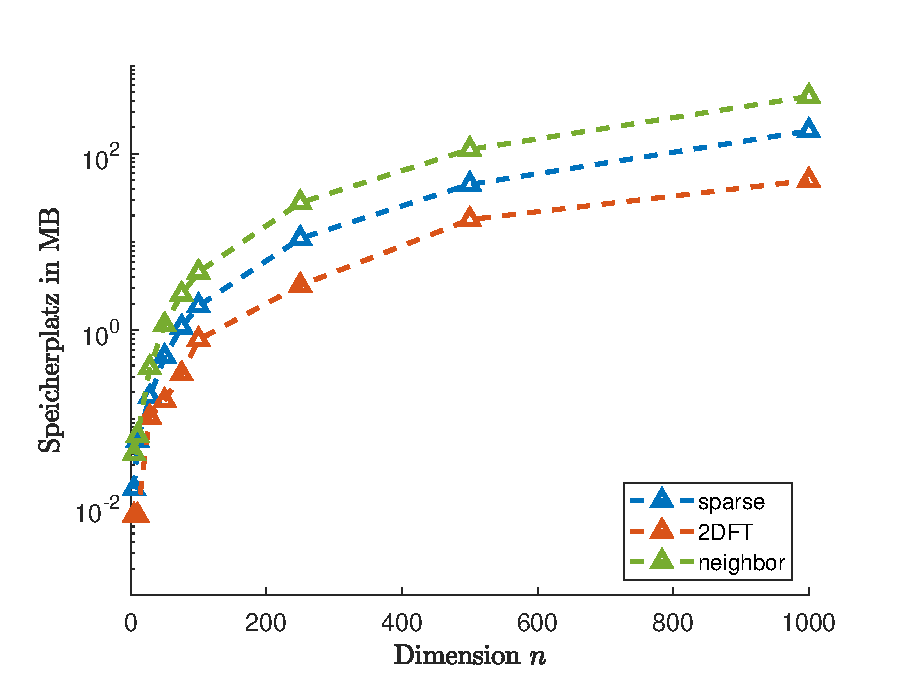
\includegraphics[width=0.8\textwidth]{pics/chapters/kap5/data_plot_vergleich_disk.eps}
    \centering
    \caption[Vergleich des zusätzlichen Speicherbedarfs]{Es ist der zusätzliche Speicherbedarf der vorgestellten Verfahren in Abhängigkeit von der Dimension $n$ abgebildet. Die blaue Kurve spiegelt den Matrixvektorprodukt-Ansatz mit dünnbesetzter Struktur wider. Die rote Kurve beschreibt den Speicherbedarf für die Matrixfaltung mithilfe der $\mathrm{2DFT}$. Mit Grün ist der Speicherbedarf des Nachbarschaft-Ansatzes in MB dargestellt.}
    \label{abb:vergleich_disk}
\end{figure}

\section{Datenbankgestützte Vorwärtsrechnung für CNN}
\label{abs_CNN_in_SQL}
In diesem Abschnitt steht das Problem \ref{prob:ffCCN} im Vordergrund und es wird eine relationale Umsetzung der Vorwärtsrechnung für ein trainiertes CNN-Modell diskutiert. In Abhängigkeit von den Hyperparameter des verwendeten Modells und dem Anwendungsszenario sind die im Abschnitt \ref{abs:conv_in_sql} vorgestellten Resultate zu nutzen.    
Die konkreten Implementierungen in SQL beziehen sich auf das im Abschnitt \ref{abs:model_mnist} vorgestellte Modell \ref{modell}, welches als laufendes Beispielmodell dienen soll. In diesem Abschnitt tauchen immer wieder Modellparameter auf, welche als trainiert und damit optimal im Sinne der gestellten Klassifikationsaufgabe vorausgesetzt werden. Nur dann ist eine sinnvolle datenbankgestützte Mustererkennung möglich.  

\subsection*{Gefaltete Übertragungsfunktion}
Bei ML-Verfahren wird oft mit mehrdimensionalen Arrays gearbeitet. Diese sind problemlos mit dem Relationenmodell vereinbar. Das Coordinate-Schema wird einfach mit entsprechenden Attributen, welche die Achsen darstellen, erweitert. Für einen Kern $K \in \RR^{q \times p \times k \times k}$ ergibt sich die Relation \textbf{K} zu

\begin{align*}
    \mathbf{K}\, ( 
    &\underline{q} \; \; \mathrm{int},\\
    &\underline{p} \; \; \mathrm{int},\\
    &\underline{i} \; \; \mathrm{int}, \\    
    &\underline{j} \; \; \mathrm{int}, \\
    &v \; \; \mathrm{double}),
\end{align*}
wobei $q$ und $p$ die neuen Achsen präsentieren. In diesem Kontext wird von einem erweiterten Coordinate-Schema gesprochen.

Zur Berechnung der Merkmalskarten durch die gefaltete Übertragungsfunktion, vgl. Definition \ref{eq:convlogit}, sind (gewichtete) Summen über Matrixfaltungen zu bestimmen. Um dies kompakt darzustellen, werden rekursive Anfragen benutzt, welche seit 1999 in SQL standardisiert sind. An dieser Stelle sei bemerkt, dass je nach Wahl des Datenbankmanagementsystems diese Anfragen unterstützt beziehungsweise nicht unterstützt werden. Ein Beispiel zur rekursiven Berechnung von
\begin{equation}
   \label{eq:sum_n}
\sum_{n=1}^{100} n    
\end{equation} 
ist in Anfrage \ref{sql:recursive} gegeben. 

\lstinputlisting[label=sql:recursive, caption=Ein Beispiel einer rekursiven SQL-Anfrage, language=SQL]{sql_code/recursive_sum_n.txt}

Eine rekursive Anfrage besteht immer aus einem nicht-rekursiven Term (im Beispiel Zeile 3), der Vereinigung \textbf{UNION} bzw. \textbf{UNION ALL} und einem rekursiven Term (Zeile 4-6), welcher den Selbstverweis auf die entsprechende Relation beinhaltet. Der \textbf{UNION ALL}-Operator entfernt im Gegensatz zum \textbf{UNION}-Operator keine Duplikate. Die erste \textbf{SELECT}-Klausel definiert die Rekursionsbasis und darf sich nicht auf die zu definierende Relation, im Beispiel \textbf{t}, beziehen. Durch diese Anweisung werden zudem die Datentypen der Attribute der zu definierenden Relation festgelegt. In den Zeilen 7 und 8 wird die Summe in Gleichung (\ref{eq:sum_n}) über die Partialsummen in der Relation \textbf{t} berechnet. 

Bei der gefalteten Übertragungsfunktion, siehe Definition \ref{eq:convlogit}, mit einer Aktivierungsfunktion $\psi$ ist eine Summe der Form
\begin{equation}
    \label{eq:rec_conv}
    \psi \left(\sum_{p=1}^{z_{in}} \alpha_{qp} A_p+ b_q \mathbf{1} \right)
\end{equation}
zu berechnen. Dabei sind die Matrizen $A_p$ Ergebnisse von Matrixfaltungen, $\alpha_{qp} \in \RR$ beliebige Gewichte sowie $b \in \RR^{z_{out}}$ ein Biasvektor. Zukünftig werden Aktivierungsfunktionen im SQL-Code mit $T$ bezeichnet. Zur Berechnung von der Summe in Gleichung (\ref{eq:rec_conv}) wird eine rekursive SQL-Anfrage \ref{sql:conv_rec} genutzt. Die entsprechenden Relationen liegen jeweils im erweiterten Coordinate-Schema vor. In der Anfrage gilt für alle Gewichte $\alpha_{qp}=1$. Die Erweiterung für beliebige Gewichte kann mit einer zusätzlichen Relation für die Gewichtsparameter gelingen. 

\lstinputlisting[label=sql:conv_rec, caption=Die rekursive SQL-Anfrage zur Berechnung der gefalteten Übertragungsfunktion, language=SQL]{sql_code/conv_recursive.txt}

Die datenbankgestützte Matrixfaltung ist bereits im vorherigen Abschnitt \ref{abs:conv_in_sql} beleuchtet worden. Zur Veranschaulichung wird die SQL-Implementierung \ref{sql:C1} zur Berechnung der sechs Merkmalskarten in der Faltungschicht $C^1$ des Modells \ref{modell} dargestellt. Dabei wurde der im Abschnitt \ref{abs:naive_app} diskutierte verbesserte Nachbarschafts-Ansatz mit Umgebungstabellen und das erweiterte Coordinate-Schema benutzt. Hier ist im Gegensatz zur Schicht $C^2$ keine rekursive Anfrage notwendig. Es kommen wieder Common-Table-Expressions zum Einsatz. In den Zeilen 1-19 werden die Matrixfaltungen $X \ast K^{1}_p$ mit zero padding mithilfe einer Umgebungstabelle \textbf{U} für $1 \leq p \leq 6$ berechnet. In den Zeilen 20 bis 27 wird nur das Teilergebnis behalten, welches mit der gültigen Faltung bestimmt wurde. Schließlich folgt in den Zeilen 28-34 die Manipulation mit den Schwellwerten $b_p$ und die Berechnung der Aktivierung mit der logistischen Funktion.

\lstinputlisting[label=sql:C1, caption=Die SQL-Anfrage zur Berechnung von $C^1$, language=SQL]{sql_code/C1_sql.txt}

\subsection*{Pooling}
Die datenbankgestützte Umsetzung von Pooling-Schichten kann direkt durch die Nutzung von Nachbarschaften wie in Abschnitt \ref{abs:naive_app} gelingen. Da die Dimensionen aller vorkommenden Merkmalskarten und Kerne eines CNN durch die Wahl der Hyperparameter festgelegt werden, müssen die Nachbarschaften beim Pooling nur einmalig berechnet werden. Des Weiteren werden Funktionen wie \textbf{MAX} und \textbf{MEAN} im SQL-Standard unterstützt, sodass Maximum-Pooling und Mittelwert-Pooling implementiert werden können.

Eine weitere Möglichkeit besteht darin, das Mittelwert-Pooling mit den Schrittweiten $p:=p_h=p_b$ als Faltungsoperation mit dem sogenannten Mittelwert-Kern $\frac{1}{p^2} \mathbf{1} \in \RR^{p \times p}$ zu implementieren. An dieser Stelle können Resultate aus dem vorherigen Abschnitt \ref{abs:conv_in_sql} genutzt werden, um abzuschätzen, welcher Ansatz für das Anwendungsszenario besser geeignet ist. Schließlich ist auch die Flatten-Funktion, vgl. Definition \ref{def:flatten}, leicht in SQL umsetzbar. 

Eine Kombination aus Mittelwert-Pooling mit Schrittweite $p=2$ und der Flatten-Funktion $T_f$ ist für das konkrete Modell \ref{modell} in der SQL-Anfrage \ref{sql:pool_flatten} gegeben. Alle beteiligten Relationen liegen entsprechend ihrer Namen im erweitertem Coordinate-Schema vor. Es wird der oben diskutierte Nachbarschaft-Ansatz gewählt.

\lstinputlisting[label=sql:pool_flatten, caption=SQL-Code zur Umsetzung des Mittelwert-Poolings und anschließender Flatten-Operation, language=SQL]{sql_code/pool_flatten.txt}

In den Zeilen 1 bis 11 wird das Mittelwert-Pooling mithilfe der Aggregatfunktion \textbf{AVG} und der Nachbarschaften in der Relation \textbf{U} bestimmt. Dieses Ergebnis wird mit den Schrittweiten $s_h=s_b=2$, vgl. Bemerkung \ref{bem_strides}, in den Zeilen 12 bis 19 in der Dimension verkleinert. Dabei werden Funktionen wie das Aufrunden \textbf{CEIL} und Modulo-Rechnen \textbf{MOD} zur passenden Selektierung der Indizes genutzt. Die Doppelpunkte sorgen dafür, dass die Indizes zu natürlichen Zahlen umgewandelt werden. Im Englischen wird diese Typumwandlung als \textit{type-casting} bezeichnet. Alle verwendeten Operationen werden im SQL-Standard unterstützt. Schließlich wird der Vektor $f=T_f(P^2) \in \RR^{192}$ der Flatten-Funktion in den Zeilen 20 bis 26 berechnet. 
 
\subsection*{Vorwärtsgerichtete neuronale Netze}
Die letzte Schicht eines CNN besteht meistens aus einem FFN mit einer oder mehreren verdeckten Neuronenschichten. Die Theorie von FFN wird in Kapitel \ref{kap:NN} vorgestellt. Dabei wird die Ausgabe eines neuronalen Netzes mittels Vorwärtsrechnung, vgl. Algorithmus \ref{alg:ff}, berechnet. Diese lässt sich ausschließlich mit bereits vorgestellten Basisoperationen wie der Matrixvektormultiplikation bzw. Vektoraddition und einfachen Funktionsauswertung darstellen. Wird das Modell \ref{modell} zur Klassifikation von Ziffern genutzt, so ist die Vorwärtsrechnung lediglich für eine Neuronenschicht datenbankgestützt umzusetzen. Die Verallgemeinerung für beliebig viele Schichten wurde bereits in einer Projektarbeit der Universität Rostock untersucht \cite{myprojekt}. 

Seien die Gewichtsmatrix $W \in \RR^{192 \times 10}$ sowie der Biasvektor $b \in \RR^{10}$ wie in Abschnitt \ref{abs:model_mnist} gegeben. Die entsprechenden Relationen \textbf{W} und \textbf{B} werden gemäß dem Coordinate-Schema erstellt. Weiter sei $T$ eine beliebige Aktivierungsfunktion. Beim Modell \ref{modell} ist $T$ die logistische Funktion. Schließlich sei für eine Eingabekarte $X$ in der Relation \textbf{FLATTEN} der Vektor $f=T_f(X)$ der Flatten-Schicht gespeichert, welcher als Eingabe des FFN dient. Die Ausgabe des FFN und damit des gesamten CNN lässt sich durch die SQL-Anfrage \ref{sql:ffn} berechnen. In den Zeilen 1-9 wird das Matrixvektorprodukt $Wf$ berechnet, welches anschließend mit dem Biasvektor $b$ manipuliert wird. Schließlich werden die Aktivierungen der Ausgabeschicht mit der Funktion $T$ ermittelt. In den Zeilen 10-15 wird der Index mit der maximalen Aktivierung selektiert, welcher, vermindert um Eins, die Klassifikation der Ziffer darstellt.

\lstinputlisting[label=sql:ffn, caption=SQL-Code zur Umsetzung der Vorwärtsrechnung des einschichtigen FFN aus Modell \ref{modell}, language=SQL]{sql_code/ffn_in_sql.txt}

Die vollständige datenbankgestützte Vorwärtsrechnung für das trainierte Modell \ref{modell} kann durch die Kombination der obigen Resultate durchgeführt werden. Für die Klassifikation von $28 \times 28$- Grauwertbildern kann wegen der Dimension der Nachbarschaft-Ansatz genutzt werden. Für andere Modelle sind je nach Anwendungsszenario und Wahl der Hyperparameter die entsprechenden Faltungs- und Pooling-Operationen mit den in Abschnitten \ref{abs:conv_in_sql} und \ref{abs_CNN_in_SQL} vorgestellten Methoden hinsichtlich deren Zeit-und Speicheraufwand umzusetzen. 